

In this section we will prove Theorem \ref{prop:stable_tame_inv}, claming that the stable
type of the assosiaded \Ainf-algebra is invarient under legendrian isotopy.

\subsection{Legendrian Reidemeister Moves}
Consider a generic Legendrien isotopy $\{L_t\}$ connecting $L_0$ and $L_1$, and
let $Y_t = \pi(L_t)$ denote the Lagrangian projection. Throughout the
deformation a finite number of bifurcations or Reidemeister moves (see Figure
\ref{fig:reid_moves} ) may occur. 
If no bifurcations occurs for $t\in[x,y]$, it is clear by the definition of the
associated \Ainf-algebra that $(A_{L_x},m_{L_x})$ and $(A_{L_y}, m_{L_y})$ are
naturally isomorphic. So In order to prove that the stable type of the
associated \Ainf-algebra is preserved throughout the isotopy, it suffices to
prove that it is preserved by the bifurcations.

\begin{figure}[h!]
\centering
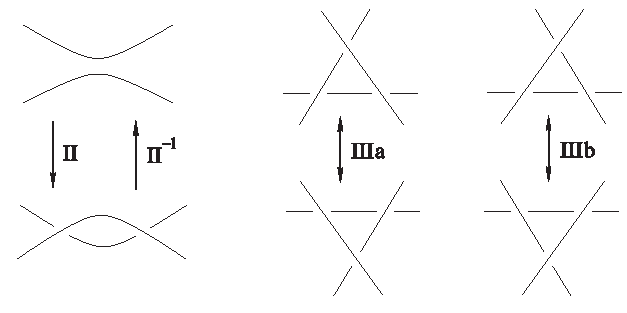
\includegraphics[width=.6\textwidth]{figs/reid_moves.pdf}
\caption{Legendrian Reidemeister Moves}
\label{fig:reid_moves}
\end{figure}

Note that the third Reidemeister move has two version, both preserving the number
of crossings, whereas the second does not. 
\comment{( The first Reidemeier move can not be realized as a Legendrian
isotopy, because it does not preserve the rotation number. )} 
We will see that for in either of the two versions of the third move the \Ainf-algebra changes by a tame isomorphism. 
In the case of the second move we will also need to stabilize, since
the number of crossings has changed.

\newcommand{\Ypm}{Y_{t'\pm\epsilon}}
\newcommand{\Yp}{Y_{t'\pm\epsilon}}
\newcommand{\Ym}{Y_{t'\pm\epsilon}}

Suppose a bifurcation occurs at $t = t'$. Consider a small $\epsilon > 0$ and let
$(A^\pm, m^\pm) = (A_{L_{t\pm\epsilon}}, m_{L_{t\pm\epsilon}})$. 
Without loss of generality, we will assume that for $t\in[t'-\epsilon, t'+\epsilon]$ the projection of the knot is unchanged
outside a small neighbourhood of where the bifurcation occurs. 


